\subsection{Motivation}


Die Workshopteilnehmer sollten zu Beginn für das Thema Affective Computing motiviert werden. Dafür gibt es einen kurze Beschreibung der Emotionen mit den Charakteristiken, wie zum Beispiel, dass Emotionen sehr schnell auftreten, aber dafür ebenfalls sehr ungenau sind\cite{emotioneninfo}. Die Intensität ist ebenfalls ein Merkmale der Emotionen. Eine hohe Intensität ist kurzzeitig und stark im Gegensatz zu einem niedrigen Intensiätsempfinden der Emotionen. Eine geringe Intensität ist dauert länger an und wird auch als Stimmung bezeichnet. 

\vspace{3mm}


	
	\begin{tabular}{c c c }
		\textbf{1 . Aufgabe} &  Zeit: 15 min & Einzelarbeit\\
	\end{tabular}

\vspace{1mm}


Ziel der Aufgabe ist es den verschiedenen Benutzerempfindlichkeiten aufzuzeigen. Die Aufgabe soll in zwei Gruppen erfolgen, bei der die Gruppen jeweils verschiedene Websiten angezeigt bekommen haben. Auf der Website sollten diese nach Informationen zu Kaffee suchen, um den veröffentlichten Fragebogen auszufüllen. Anschließend sollten die Emotionen eingetragen werden. Während Gruppe 1 ihre Informationen in Wikipedia recherchierte\cite{kaffeewiki}, durfte Gruppe 2 eine Website besuchen, welche den Inhalt grafisch ergänzt\cite{kaffecss}. Dabei zeigte sich folgende Auswertungen der Emotionen, welche in Abbildung 1 und Abbildung 2 dargestellt.


\begin{figure}[!h]
	\centering
	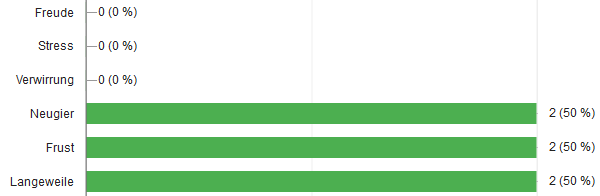
\includegraphics[width=0.9\linewidth]{Pictures/wiki_kaffee}
	\caption[Ergebnis der grafischen Website]{Ergebnis von Wikipedia}
	\label{fig:ergebnis_1}
\end{figure}

\begin{figure}[!h]
	\centering
	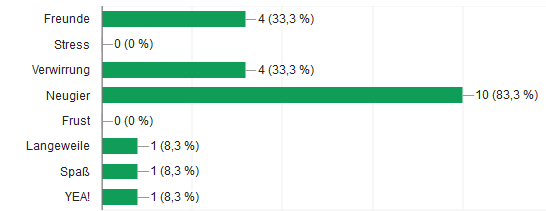
\includegraphics[width=0.9\linewidth]{Pictures/bizbuzz}
	\caption[Ergebnis von Wikipedia]{Ergebnis von Wikipedia}
	\label{fig:ergebnis_2}
\end{figure}


Die Ergebnisse wurden den Gruppen vorgestellt mit dem Verweise, dass Benutzer verschieden sind und anders empfinden. Schließlich stellten wir eine möglich Erklärung diese Verhalten vor, indem wir den Kontext einer Person erläuterten. Der Kontext einer Person ist sehr umfangreich. Als Beispiel sind hierfür der kulturelle Hintergrund, die eigenen Interessen und Hobbys sowie das soziale Umfeld zu nennen.  




